\documentclass[10pt]{article}
\usepackage[polish]{babel}
\usepackage[utf8]{inputenc}
\usepackage[T1]{fontenc}
\usepackage{graphicx}
\usepackage[export]{adjustbox}
\graphicspath{ {./images/} }
\usepackage{amsmath}
\usepackage{amsfonts}
\usepackage{amssymb}
\usepackage[version=4]{mhchem}
\usepackage{stmaryrd}
\usepackage{multirow}

\title{EGZAMIN MATURALNY Z MATEMATYKI }

\author{}
\date{}


\begin{document}
\maketitle
Arkusz zawiera informacje prawnie chronione do momentu rozpoczęcia egzaminu.

KOD\\
PESEL\\
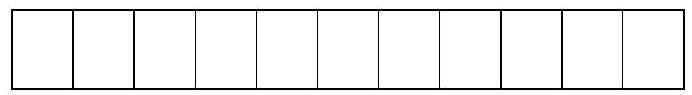
\includegraphics[max width=\textwidth, center]{2024_11_21_85128ec2a66a58098779g-01}\\
\(\square\)

\section*{POZIOM ROZSZERZONY}
\section*{Instrukcja dla zdającego}
\begin{enumerate}
  \item Sprawdź, czy arkusz egzaminacyjny zawiera 24 strony (zadania 1-11). Ewentualny brak zgłoś przewodniczącemu zespołu nadzorującego egzamin.
  \item Rozwiązania zadań i odpowiedzi wpisuj w miejscu na to przeznaczonym.
  \item Pamiętaj, że pominięcie argumentacji lub istotnych obliczeń w rozwiązaniu zadania otwartego może spowodować, że za to rozwiązanie nie otrzymasz pełnej liczby punktów.
  \item Pisz czytelnie i używaj tylko długopisu lub pióra z czarnym tuszem lub atramentem.
  \item Nie używaj korektora, a błędne zapisy wyraźnie przekreśl.
  \item Pamiętaj, że zapisy w brudnopisie nie będą oceniane.
  \item Możesz korzystać z zestawu wzorów matematycznych, cyrkla i linijki oraz kalkulatora prostego.
  \item Na tej stronie oraz na karcie odpowiedzi wpisz swój numer PESEL i przyklej naklejkę z kodem.
  \item Nie wpisuj żadnych znaków w części przeznaczonej dla egzaminatora.
\end{enumerate}

UZUPELNIA ZESPÓŁ NADZORUJĄCY\\
Uprawnienia zdającego do:\\

\includegraphics[max width=\textwidth, center]{2024_11_21_85128ec2a66a58098779g-01(1)}\\
dostosowania kryteriów ocenianianieprzenoszenia zaznaczeń na kartę

9 MAJA 2019

Godzina rozpoczęcia:\\
9:00

Czas pracy:\\
180 minut

Liczba punktów do uzyskania: 50

MMA-R1\_1P-192

\section*{Zadanie 1. (5 pkt)}
Funkcja \(f\) jest określona wzorem \(f(x)=\frac{|x+2|}{x+2}-x+3|x-1|\), dla każdej liczby rzeczywistej \(x \neq-2\). Wyznacz zbiór wartości tej funkcji.\\

\includegraphics[max width=\textwidth, center]{2024_11_21_85128ec2a66a58098779g-02}\\

\includegraphics[max width=\textwidth, center]{2024_11_21_85128ec2a66a58098779g-03}

Odpowiedź:

\begin{center}
\begin{tabular}{|c|l|c|}
\hline
\multirow{2}{*}{\begin{tabular}{l}
Wypelnia \\
egzaminator \\
\end{tabular}} & Nr zadania & 1. \\
\cline { 2 - 3 }
 & Maks. liczba pkt & 5 \\
\cline { 2 - 3 }
 & Uzyskana liczba pkt &  \\
\hline
\end{tabular}
\end{center}

\section*{Zadanie 2. (3 pkt)}
Udowodnij, że dla dowolnych dodatnich liczb rzeczywistych \(x\) i \(y\), takich że \(x<y\), i dowolnej dodatniej liczby rzeczywistej \(a\) prawdziwa jest nierówność \(\frac{x+a}{y+a}+\frac{y}{x}>2\).

\begin{center}
\begin{tabular}{|c|c|c|c|c|c|c|c|c|c|c|c|c|c|c|c|c|c|c|c|c|c|c|}
\hline
 &  &  &  &  &  &  &  &  &  &  &  &  &  &  &  &  &  &  &  &  &  &  \\
\hline
 &  &  &  &  &  &  &  &  &  &  &  &  &  &  &  &  &  &  &  &  &  &  \\
\hline
 &  &  &  &  &  &  &  &  &  &  &  &  &  &  &  &  &  &  &  &  &  &  \\
\hline
 &  &  &  &  &  &  &  &  &  &  &  &  &  &  &  &  &  &  &  &  &  &  \\
\hline
 &  &  &  &  &  &  &  &  &  &  &  &  &  &  &  &  &  &  &  &  &  &  \\
\hline
 &  &  &  &  &  &  &  &  &  &  &  &  &  &  &  &  &  &  &  &  &  &  \\
\hline
 &  &  &  &  &  &  &  &  &  &  &  &  &  &  &  &  &  &  &  &  &  &  \\
\hline
 &  &  &  &  &  &  &  &  &  &  &  &  &  &  &  &  &  &  &  &  &  &  \\
\hline
 &  &  &  &  &  &  &  &  &  &  &  &  &  &  &  &  &  &  &  &  &  &  \\
\hline
 &  &  &  &  &  &  &  &  &  &  &  &  &  &  &  &  &  &  &  &  &  &  \\
\hline
 &  &  &  &  &  &  &  &  &  &  &  &  &  &  &  &  &  &  &  &  &  &  \\
\hline
 &  &  &  &  &  &  &  &  &  &  &  &  &  &  &  &  &  &  &  &  &  &  \\
\hline
 &  &  &  &  &  &  &  &  &  &  &  &  &  &  &  &  &  &  &  &  &  &  \\
\hline
 &  &  &  &  &  &  &  &  &  &  &  &  &  &  &  &  &  &  &  &  &  &  \\
\hline
 &  &  &  &  &  &  &  &  &  &  &  &  &  &  &  &  &  &  &  &  &  &  \\
\hline
 &  &  &  &  &  &  &  &  &  &  &  &  &  &  &  &  &  &  &  &  &  &  \\
\hline
 &  &  &  &  &  &  &  &  &  &  &  &  &  &  &  &  &  &  &  &  &  &  \\
\hline
 &  &  &  &  &  &  &  &  &  &  &  &  &  &  &  &  &  &  &  &  &  &  \\
\hline
 &  &  &  &  &  &  &  &  &  &  &  &  &  &  &  &  &  &  &  &  &  &  \\
\hline
 &  &  &  &  &  &  &  &  &  &  &  &  &  &  &  &  &  &  &  &  &  &  \\
\hline
 &  &  &  &  &  &  &  &  &  &  &  &  &  &  &  &  &  &  &  &  &  &  \\
\hline
 &  &  &  &  &  &  &  &  &  &  &  &  &  &  &  &  &  &  &  &  &  &  \\
\hline
 &  &  &  &  &  &  &  &  &  &  &  &  &  &  &  &  &  &  &  &  &  &  \\
\hline
 &  &  &  &  &  &  &  &  &  &  &  &  &  &  &  &  &  &  &  &  &  &  \\
\hline
 &  &  &  &  &  &  &  &  &  &  &  &  &  &  &  &  &  &  &  &  &  &  \\
\hline
 &  &  &  &  &  &  &  &  &  &  &  &  &  &  &  &  &  &  &  &  &  &  \\
\hline
 &  &  &  &  &  &  &  &  &  &  &  &  &  &  &  &  &  &  &  &  &  &  \\
\hline
 &  &  &  &  &  &  &  &  &  &  &  &  &  &  &  &  &  &  &  &  &  &  \\
\hline
 &  &  &  &  &  &  &  &  &  &  &  &  &  &  &  &  &  &  &  &  &  &  \\
\hline
 &  &  &  &  &  &  &  &  &  &  &  &  &  &  &  &  &  &  &  &  &  &  \\
\hline
 &  &  &  &  &  &  &  &  &  &  &  &  &  &  &  &  &  &  &  &  &  &  \\
\hline
 &  &  &  &  &  &  &  &  &  &  &  &  &  &  &  &  &  &  &  &  &  &  \\
\hline
 &  &  &  &  &  &  &  &  &  &  &  &  &  &  &  &  &  &  &  &  &  &  \\
\hline
 &  &  &  &  &  &  &  &  &  &  &  &  &  &  &  &  &  &  &  &  &  &  \\
\hline
 &  &  &  &  &  &  &  &  &  &  &  &  &  &  &  &  &  &  &  &  &  &  \\
\hline
 &  &  &  &  &  &  &  &  &  &  &  &  &  &  &  &  &  &  &  &  &  &  \\
\hline
 &  &  &  &  &  &  &  &  &  &  &  &  &  &  &  &  &  &  &  &  &  &  \\
\hline
 &  &  &  &  &  &  &  &  &  &  &  &  &  &  &  &  &  &  &  &  &  &  \\
\hline
 &  &  &  &  &  &  &  &  &  &  &  &  &  &  &  &  &  &  &  &  &  &  \\
\hline
 &  &  &  &  &  &  &  &  &  &  &  &  &  &  &  &  &  &  &  &  &  &  \\
\hline
 &  &  &  &  &  &  &  &  &  &  &  &  &  &  &  &  &  &  &  &  &  &  \\
\hline
 &  &  &  &  &  &  &  &  &  &  &  &  &  &  &  &  &  &  &  &  &  &  \\
\hline
 &  &  &  &  &  &  &  &  &  &  &  &  &  &  &  &  &  &  &  &  &  &  \\
\hline
\end{tabular}
\end{center}

\begin{center}

\includegraphics[max width=\textwidth]{2024_11_21_85128ec2a66a58098779g-05}
\end{center}

\begin{center}
\begin{tabular}{|c|l|c|}
\hline
\multirow{2}{*}{\begin{tabular}{l}
Wypelnia \\
egzaminator \\
\end{tabular}} & Nr zadania & 2. \\
\cline { 2 - 3 }
 & Maks. liczba pkt & \(\mathbf{3}\) \\
\cline { 2 - 3 }
 & Uzyskana liczba pkt &  \\
\hline
\end{tabular}
\end{center}

\section*{Zadanie 3. (3 pkt)}
Dany jest trójkąt równoramienny \(A B C\), w którym \(|A C|=|B C|\). Na ramieniu \(A C\) tego trójkąta wybrano punkt \(M(M \neq A\) i \(M \neq C)\), a na ramieniu \(B C\) wybrano punkt \(N\), w taki sposób, że \(|A M|=|C N|\). Przez punkty \(M\) i \(N\) poprowadzono proste prostopadłe do podstawy \(A B\) tego trójkąta, które wyznaczają na niej punkty \(S\) i \(T\). Udowodnij, że \(|S T|=\frac{1}{2}|A B|\).\\

\includegraphics[max width=\textwidth, center]{2024_11_21_85128ec2a66a58098779g-06}\\

\includegraphics[max width=\textwidth, center]{2024_11_21_85128ec2a66a58098779g-07}

\begin{center}
\begin{tabular}{|c|l|c|}
\hline
\multirow{2}{*}{\begin{tabular}{c}
Wypetnia \\
egzaminator \\
\end{tabular}} & Nr zadania & \(\mathbf{3 .}\) \\
\cline { 2 - 3 }
 & Maks. liczba pkt & \(\mathbf{3}\) \\
\cline { 2 - 3 }
 & Uzyskana liczba pkt &  \\
\hline
\end{tabular}
\end{center}

\section*{Zadanie 4. (5 pkt)}
Ciąg \((a, b, c)\) jest geometryczny, ciąg \((a+1, b+5, c)\) jest malejącym ciągiem arytmetycznym oraz \(a+b+c=39\). Oblicz \(a, b, c\).\\

\includegraphics[max width=\textwidth, center]{2024_11_21_85128ec2a66a58098779g-08}\\

\includegraphics[max width=\textwidth, center]{2024_11_21_85128ec2a66a58098779g-09}

Odpowiedź: \(\qquad\)

\begin{center}
\begin{tabular}{|c|l|c|}
\hline
\multirow{2}{*}{\begin{tabular}{l}
Wypetnia \\
egzaminator \\
\end{tabular}} & Nr zadania & 4. \\
\cline { 2 - 3 }
 & Maks. liczba pkt & 5 \\
\cline { 2 - 3 }
 & Uzyskana liczba pkt &  \\
\hline
\end{tabular}
\end{center}

\section*{Zadanie 5. (6 pkt)}
Dane są okręgi o równaniach \(x^{2}+y^{2}-12 x-8 y+43=0\) i \(x^{2}+y^{2}-2 a x+4 y+a^{2}-77=0\). Wyznacz wszystkie wartości parametru \(a\), dla których te okręgi mają dokładnie jeden punkt wspólny. Rozważ wszystkie przypadki.\\

\includegraphics[max width=\textwidth, center]{2024_11_21_85128ec2a66a58098779g-10}\\

\includegraphics[max width=\textwidth, center]{2024_11_21_85128ec2a66a58098779g-11}

Odpowiedź: \(\qquad\)

\begin{center}
\begin{tabular}{|c|l|c|}
\hline
\multirow{2}{*}{\begin{tabular}{c}
Wypetnia \\
egzaminator \\
\end{tabular}} & Nr zadania & 5. \\
\cline { 2 - 3 }
 & Maks. liczba pkt & 6 \\
\cline { 2 - 3 }
 & Uzyskana liczba pkt &  \\
\hline
\end{tabular}
\end{center}

\section*{Zadanie 6. (5 pht)}
Wielomian określony wzorem \(W(x)=2 x^{3}+\left(m^{3}+2\right) x^{2}-11 x-2(2 m+1)\) jest podzielny przez dwumian \((x-2)\) oraz przy dzieleniu przez dwumian \((x+1)\) daje resztę 6 . Oblicz \(m\) oraz pierwiastki wielomianu \(W\) dla wyznaczonej wartości \(m\).\\

\includegraphics[max width=\textwidth, center]{2024_11_21_85128ec2a66a58098779g-12}\\

\includegraphics[max width=\textwidth, center]{2024_11_21_85128ec2a66a58098779g-13}

Odpowiedź:

\begin{center}
\begin{tabular}{|c|l|c|}
\hline
\multirow{2}{*}{\begin{tabular}{l}
Wypelnia \\
egzaminator \\
\end{tabular}} & Nr zadania & \(\mathbf{6 .}\) \\
\cline { 2 - 3 }
 & Maks. liczba pkt & 5 \\
\cline { 2 - 3 }
 & Uzyskana liczba pkt &  \\
\hline
\end{tabular}
\end{center}

\section*{Zadanie 7. (4 pkt)}
Rozwiąż równanie \(\cos 2 x=\sin x+1 \mathrm{w}\) przedziale \(\langle 0,2 \pi\rangle\).\\

\includegraphics[max width=\textwidth, center]{2024_11_21_85128ec2a66a58098779g-14}\\

\includegraphics[max width=\textwidth, center]{2024_11_21_85128ec2a66a58098779g-15}

Odpowiedź: \(\qquad\)

\begin{center}
\begin{tabular}{|c|l|c|}
\hline
\multirow{2}{*}{\begin{tabular}{l}
Wypelnia \\
egzaminator \\
\end{tabular}} & Nr zadania & 7. \\
\cline { 2 - 3 }
 & Maks. liczba pkt & 4 \\
\cline { 2 - 3 }
 & Uzyskana liczba pkt &  \\
\hline
\end{tabular}
\end{center}

\section*{Zadanie 8. (4 pht)}
Punkt \(D\) leży na boku \(A B\) trójkąta \(A B C\) oraz \(|A C|=16,|A D|=6,|C D|=14\) i \(|B C|=|B D|\). Oblicz obwód trójkąta \(A B C\).\\

\includegraphics[max width=\textwidth, center]{2024_11_21_85128ec2a66a58098779g-16}\\

\includegraphics[max width=\textwidth, center]{2024_11_21_85128ec2a66a58098779g-17}

Odpowiedź:

\begin{center}
\begin{tabular}{|c|l|c|}
\hline
\multirow{2}{*}{\begin{tabular}{l}
Wypelnia \\
egzaminator \\
\end{tabular}} & Nr zadania & 8. \\
\cline { 2 - 3 }
 & Maks. liczba pkt & 4 \\
\cline { 2 - 3 }
 & Uzyskana liczba pkt &  \\
\hline
\end{tabular}
\end{center}

\section*{Zadanie 9. (6 pht)}
Wyznacz wszystkie wartości parametru \(m\), dla których funkcja kwadratowa \(f\) określona wzorem

\[
f(x)=(2 m+1) x^{2}+(m+2) x+m-3
\]

ma dwa różne pierwiastki rzeczywiste \(x_{1}, x_{2}\) spełniające warunek \(\left(x_{1}-x_{2}\right)^{2}+5 x_{1} x_{2} \geq 1\).

\begin{center}
\begin{tabular}{|c|c|c|c|c|c|c|c|c|c|c|c|c|c|c|c|c|c|c|c|c|c|c|}
\hline
 &  &  &  &  &  &  &  &  &  &  &  &  &  &  &  &  &  &  &  &  &  &  \\
\hline
 &  &  &  &  &  &  &  &  &  &  &  &  &  &  &  &  &  &  &  &  &  &  \\
\hline
 &  &  &  &  &  &  &  &  &  &  &  &  &  &  &  &  &  &  &  &  &  &  \\
\hline
 &  &  &  &  &  &  &  &  &  &  &  &  &  &  &  &  &  &  &  &  &  &  \\
\hline
 &  &  &  &  &  &  &  &  &  &  &  &  &  &  &  &  &  &  &  &  &  &  \\
\hline
 &  &  &  &  &  &  &  &  &  &  &  &  &  &  &  &  &  &  &  &  &  &  \\
\hline
 &  &  &  &  &  &  &  &  &  &  &  &  &  &  &  &  &  &  &  &  &  &  \\
\hline
 &  &  &  &  &  &  &  &  &  &  &  &  &  &  &  &  &  &  &  &  &  &  \\
\hline
 &  &  &  &  &  &  &  &  &  &  &  &  &  &  &  &  &  &  &  &  &  &  \\
\hline
 &  &  &  &  &  &  &  &  &  &  &  &  &  &  &  &  &  &  &  &  &  &  \\
\hline
 &  &  &  &  &  &  &  &  &  &  &  &  &  &  &  &  &  &  &  &  &  &  \\
\hline
 &  &  &  &  &  &  &  &  &  &  &  &  &  &  &  &  &  &  &  &  &  &  \\
\hline
 &  &  &  &  &  &  &  &  &  &  &  &  &  &  &  &  &  &  &  &  &  &  \\
\hline
 &  &  &  &  &  &  &  &  &  &  &  &  &  &  &  &  &  &  &  &  &  &  \\
\hline
 &  &  &  &  &  &  &  &  &  &  &  &  &  &  &  &  &  &  &  &  &  &  \\
\hline
 &  &  &  &  &  &  &  &  &  &  &  &  &  &  &  &  &  &  &  &  &  &  \\
\hline
 &  &  &  &  &  &  &  &  &  &  &  &  &  &  &  &  &  &  &  &  &  &  \\
\hline
 &  &  &  &  &  &  &  &  &  &  &  &  &  &  &  &  &  &  &  &  &  &  \\
\hline
 &  &  &  &  &  &  &  &  &  &  &  &  &  &  &  &  &  &  &  &  &  &  \\
\hline
 &  &  &  &  &  &  &  &  &  &  &  &  &  &  &  &  &  &  &  &  &  &  \\
\hline
 &  &  &  &  &  &  &  &  &  &  &  &  &  &  &  &  &  &  &  &  &  &  \\
\hline
 &  &  &  &  &  &  &  &  &  &  &  &  &  &  &  &  &  &  &  &  &  &  \\
\hline
 &  &  &  &  &  &  &  &  &  &  &  &  &  &  &  &  &  &  &  &  &  &  \\
\hline
 &  &  &  &  &  &  &  &  &  &  &  &  &  &  &  &  &  &  &  &  &  &  \\
\hline
 &  &  &  &  &  &  &  &  &  &  &  &  &  &  &  &  &  &  &  &  &  &  \\
\hline
 &  &  &  &  &  &  &  &  &  &  &  &  &  &  &  &  &  &  &  &  &  &  \\
\hline
 &  &  &  &  &  &  &  &  &  &  &  &  &  &  &  &  &  &  &  &  &  &  \\
\hline
 &  &  &  &  &  &  &  &  &  &  &  &  &  &  &  &  &  &  &  &  &  &  \\
\hline
 &  &  &  &  &  &  &  &  &  &  &  &  &  &  &  &  &  &  &  &  &  &  \\
\hline
 &  &  &  &  &  &  &  &  &  &  &  &  &  &  &  &  &  &  &  &  &  &  \\
\hline
 &  &  &  &  &  &  &  &  &  &  &  &  &  &  &  &  &  &  &  &  &  &  \\
\hline
 &  &  &  &  &  &  &  &  &  &  &  &  &  &  &  &  &  &  &  &  &  &  \\
\hline
 &  &  &  &  &  &  &  &  &  &  &  &  &  &  &  &  &  &  &  &  &  &  \\
\hline
 &  &  &  &  &  &  &  &  &  &  &  &  &  &  &  &  &  &  &  &  &  &  \\
\hline
 &  &  &  &  &  &  &  &  &  &  &  &  &  &  &  &  &  &  &  &  &  &  \\
\hline
 &  &  &  &  &  &  &  &  &  &  &  &  &  &  &  &  &  &  &  &  &  &  \\
\hline
 &  &  &  &  &  &  &  &  &  &  &  &  &  &  &  &  &  &  &  &  &  &  \\
\hline
 &  &  &  &  &  &  &  &  &  &  &  &  &  &  &  &  &  &  &  &  &  &  \\
\hline
 &  &  &  &  &  &  &  &  &  &  &  &  &  &  &  &  &  &  &  &  &  &  \\
\hline
 &  &  &  &  &  &  &  &  &  &  &  &  &  &  &  &  &  &  &  &  &  &  \\
\hline
 &  &  &  &  &  &  &  &  &  &  &  &  &  &  &  &  &  &  &  &  &  &  \\
\hline
 &  &  &  &  &  &  &  &  &  &  &  &  &  &  &  &  &  &  &  &  &  &  \\
\hline
\end{tabular}
\end{center}

\begin{center}

\includegraphics[max width=\textwidth]{2024_11_21_85128ec2a66a58098779g-19}
\end{center}

Odpowiedź:

\begin{center}
\begin{tabular}{|c|l|c|}
\hline
\multirow{2}{*}{\begin{tabular}{c}
Wypelnia \\
egzaminator \\
\end{tabular}} & Nr zadania & 9. \\
\cline { 2 - 3 }
 & Maks. liczba pkt & 6 \\
\cline { 2 - 3 }
 & Uzyskana liczba pkt &  \\
\hline
\end{tabular}
\end{center}

\section*{Zadanie 10. (3 pkt)}
Ze zbioru \(\{1,2,3,4,5,6,7,8,9\}\) losujemy kolejno ze zwracaniem trzy liczby. Oblicz prawdopodobieństwo zdarzenia polegającego na tym, że dokładnie dwie spośród trzech wylosowanych liczb będą równe. Wynik zapisz w postaci ułamka nieskracalnego.\\

\includegraphics[max width=\textwidth, center]{2024_11_21_85128ec2a66a58098779g-20}\\

\includegraphics[max width=\textwidth, center]{2024_11_21_85128ec2a66a58098779g-21}

Odpowiedź: \(\qquad\)

\begin{center}
\begin{tabular}{|c|l|c|}
\hline
\multirow{2}{*}{\begin{tabular}{l}
Wypelnia \\
egzaminator \\
\end{tabular}} & Nr zadania & 10. \\
\cline { 2 - 3 }
 & Maks. liczba pkt & \(\mathbf{3}\) \\
\cline { 2 - 3 }
 & Uzyskana liczba pkt &  \\
\hline
\end{tabular}
\end{center}

\section*{Zadanie 11. (6 pkt)}
Podstawą ostrosłupa \(A B C D S\) jest prostokąt \(A B C D\), którego boki mają długości \(|A B|=32\)\\
i \(|B C|=18\). Ściany boczne \(A B S\) i \(C D S\) są trójkątami przystającymi i każda z nich jest nachylona do płaszczyzny podstawy ostrosłupa pod kątem \(\alpha\). Ściany boczne \(B C S\) i \(A D S\) są trójkątami przystającymi i każda z nich jest nachylona do płaszczyzny podstawy pod kątem \(\beta\). Miary kątów \(\alpha\) i \(\beta\) spełniają warunek: \(\alpha+\beta=90^{\circ}\). Oblicz pole powierzchni całkowitej tego ostrosłupa.\\

\includegraphics[max width=\textwidth, center]{2024_11_21_85128ec2a66a58098779g-22}\\

\includegraphics[max width=\textwidth, center]{2024_11_21_85128ec2a66a58098779g-23}

Odpowiedź:

\begin{center}
\begin{tabular}{|c|l|c|}
\hline
\multirow{2}{*}{\begin{tabular}{l}
Wypelnia \\
egzaminator \\
\end{tabular}} & Nr zadania & 11. \\
\cline { 2 - 3 }
 & Maks. liczba pkt & 6 \\
\cline { 2 - 3 }
 & Uzyskana liczba pkt &  \\
\hline
\end{tabular}
\end{center}

\section*{BRUDNOPIS (nie podlega ocenie)}

\end{document}